\section{Results}\label{sec:results}


We evaluate the method on three Alpine glaciers spanning a wide range of size and
data availability. Argentière (French Alps) serves as a
benchmark: among the most densely monitored glaciers in the world, it combines a
long GLACIOCLIM stake record, repeated ground-penetrating-radar surveys and a
high-resolution Pléiades archive, and it is the subject of the state-of-the-art
distributed reconstruction of \citet{kneib2024}, against which we compare
directly. The Great Aletsch and Rhône (Swiss Alps) represent the operational regime
the method is ultimately intended for: neither has thickness soundings, so the
data assimilation is constrained by surface velocity alone, and both are
validated against raw stake measurements only.

The results are presented in three parts. We first report the Argentière
benchmark---the calibrated dynamical state, and the inferred SMB profile with its
validation against the GLACIOCLIM network
(Sects~\ref{sec:argentiere-da}--\ref{sec:inferred}). We then apply the
identical pipeline, without re-tuning, to the two velocity-only glaciers
(Sect.~\ref{sec:transfer}). Finally, we use these glaciers to quantify the
sensitivity of the inferred SMB to the basal sliding coefficient---the dynamical
parameter least constrained in the absence of thickness data
(Sect.~\ref{sec:sensitivity}).

\subsection{Calibrated ice-dynamics state}\label{sec:argentiere-da}

On Argentière the data assimilation jointly retrieves the ice-thickness field
$H_\mathrm{DA}$ and a basal-sliding field $c_\mathrm{DA}$ that reproduce both the
observed surface velocity and the GPR thickness transects, converging within
$10^2$ L-BFGS iterations (Fig.~\ref{fig:da}). Modelled velocities match the
observations to a root-mean-square residual of $3\,\mathrm{m\,yr^{-1}}$, an order
of magnitude below typical trunk velocities ($20$--$80\,\mathrm{m\,yr^{-1}}$,
locally exceeding $150\,\mathrm{m\,yr^{-1}}$ on the Rognons confluence), and the
calibrated thickness departs from the GPR transects by $\mathrm{RMS}=12\,\mathrm{m}$
(bias $-9\,\mathrm{m}$), of the order of the GPR uncertainty itself
\citep{rabatel2018}. The sliding field shows the expected structure, enhanced along
the central flowline and reduced near the lateral margins.

This calibrated state fixes the bedrock through Eqn.~(\ref{eq:bed}) and provides the
frozen dynamical substrate for the transient forward run (Sect.~\ref{sec:inference}).
Integrated forward for one year under zero SMB it produces no spurious thickness
drift, confirming that it is in mechanical equilibrium and that any subsequent
geometry change is attributable to the prescribed SMB rather than to residual model
imbalance.

% --- FIGURE PLACEHOLDER -------------------------------------------------
\begin{figure}
    \centering
    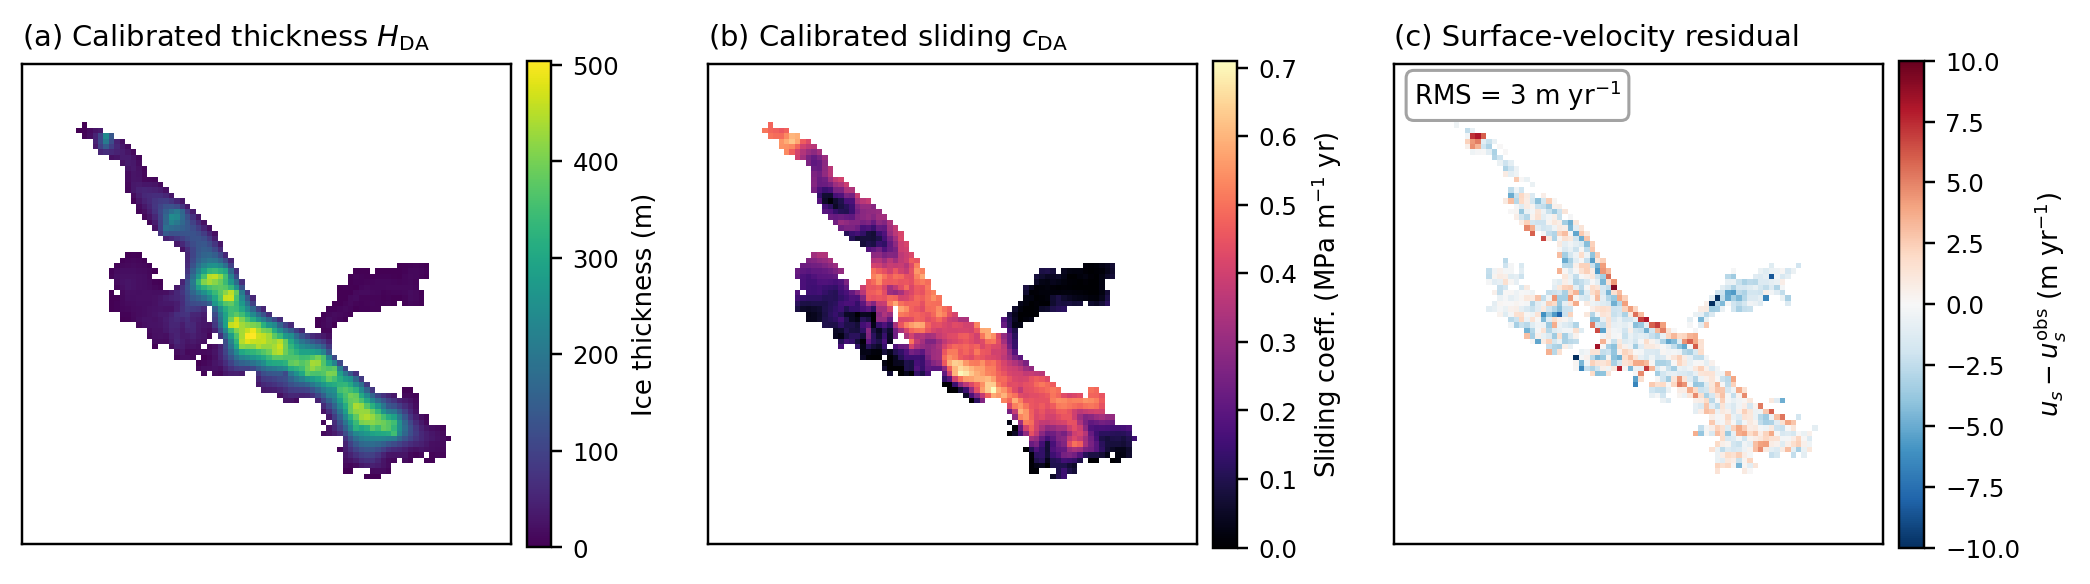
\includegraphics[width=\linewidth]{figs/argentiere_da_panel.png}
    \caption{Calibrated data-assimilation state on Argentière Glacier at
    $t_0 = 2012$. (a)~Calibrated ice thickness $H_\mathrm{DA}$ and
    (b)~calibrated basal-sliding field $c_\mathrm{DA}$, the frozen dynamical
    state passed to the SMB inversion. (c)~Surface-velocity residual
    $u_s - u_s^\mathrm{obs}$, near zero across the glacier (overall
    $\mathrm{RMS} = 3\,\mathrm{m\,yr^{-1}}$); white cells lack a velocity
    observation.}
    \label{fig:da}
\end{figure}
% ------------------------------------------------------------------------

\subsection{Inferred SMB and validation}
\label{sec:inferred}

Holding $(H_\mathrm{DA}, c_\mathrm{DA})$ fixed, we run the transient forward
simulation from 2012 to 2021 and invert for the elevation-resolved SMB profile
$\beta(z)$ that minimises the geometry-misfit cost (Eqn.~\ref{eq:cost}); the L-BFGS
optimiser converges in $\mathcal{O}(50)$ function evaluations.
The retrieved profile (Fig.~\ref{fig:smb_profile}) increases across the full altitudinal
range of the glacier (1670--3610\,m\,a.s.l.), from strongly negative values at the
tongue ($-8.5\,\mathrm{m\,w.e.\,yr^{-1}}$ at $1700\,\mathrm{m}$) to a positive
accumulation regime in the upper basin, and the simulated end-of-window thickness
$H^\mathrm{sim}(\cdot, T)$ matches the target $H^\mathrm{obs}(\cdot, T)$ across the
trunk to within the DEM differencing uncertainty (Fig.~\ref{fig:thk-comp}).

Validated against the GLACIOCLIM network---$\beta(z)$ sampled at the elevation of
each stake on the main trunk and the Améthystes tributary, compared with the
2012--2021 mean stake measurements---the inferred profile reproduces the observed
altitudinal pattern (Fig.~\ref{fig:smb_profile}) with a root-mean-square error of
$0.454\,\mathrm{m\,w.e.\,yr^{-1}}$ (Table~\ref{tab:rmse}), lower than every
previously published distributed reconstruction on this site over this period: the
F2019, SIA and IGM-distributed approaches of \citet{kneib2024} report $0.50$,
$0.67$ and $0.85\,\mathrm{m\,w.e.\,yr^{-1}}$ against the same stakes. Because the
inversion variable is one-dimensional, horizontal heterogeneity within an elevation
band---notably the avalanche-fed accumulation hotspots reported by
\citet{kneib2024}---is not resolved, consistent with the spatially structured
thickness residual in Fig.~\ref{fig:thk-comp}(c). This deliberate trade-off, which
buys a tuning-free and transferable inversion, is taken up in
Sect.~\ref{sec:discussion}.

A central feature of the method is that the flux divergence is recomputed at every
time step from the evolving geometry, rather than held stationary at a single
snapshot as in geodetic SMB inversions \citep{kneib2024, miles2021}. The bias this
stationarity assumption would introduce is quantified directly against in situ
stakes on the two velocity-only glaciers in Sect.~\ref{sec:transfer}
(Fig.~\ref{fig:smb-continuity}).

\begin{figure}
    \centering
    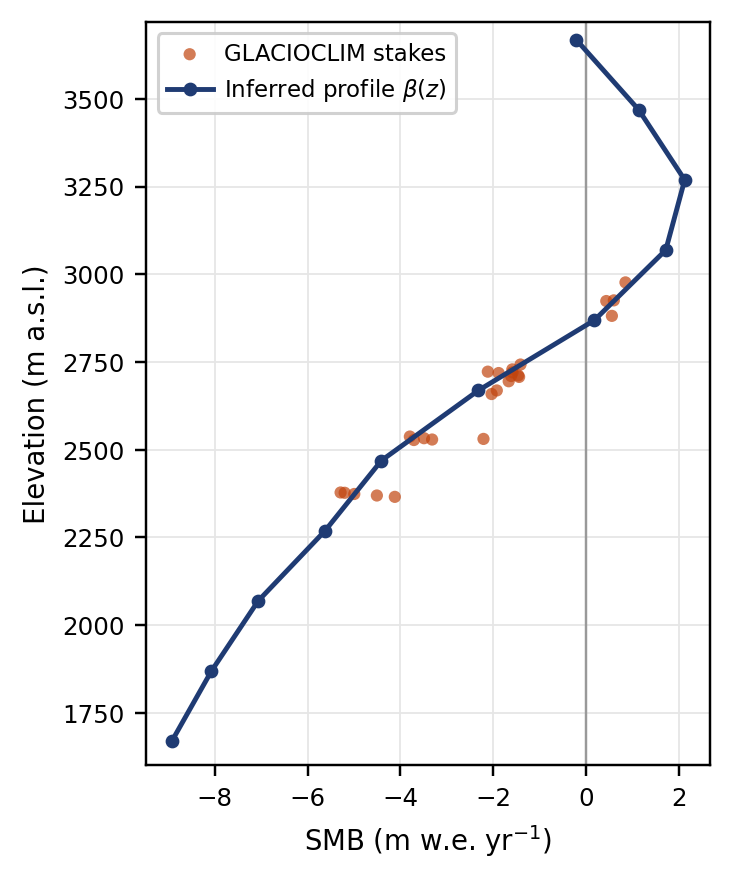
\includegraphics[width=0.5\linewidth]{figs/argentiere_smb_profile.png}
    \caption{Inferred elevation-resolved SMB profile $\beta(z)$ (blue line) for
    Argentière Glacier over 2012--2021, in water equivalent. Orange dots are the
    2012--2021 mean GLACIOCLIM stake balances, plotted at the elevation of each
    stake. The profile is sampled at 11 elevation bins of $200\,\mathrm{m}$ width
    spanning 1670--3610\,m\,a.s.l.}
    \label{fig:smb_profile}
\end{figure}

\begin{figure}
    \centering
    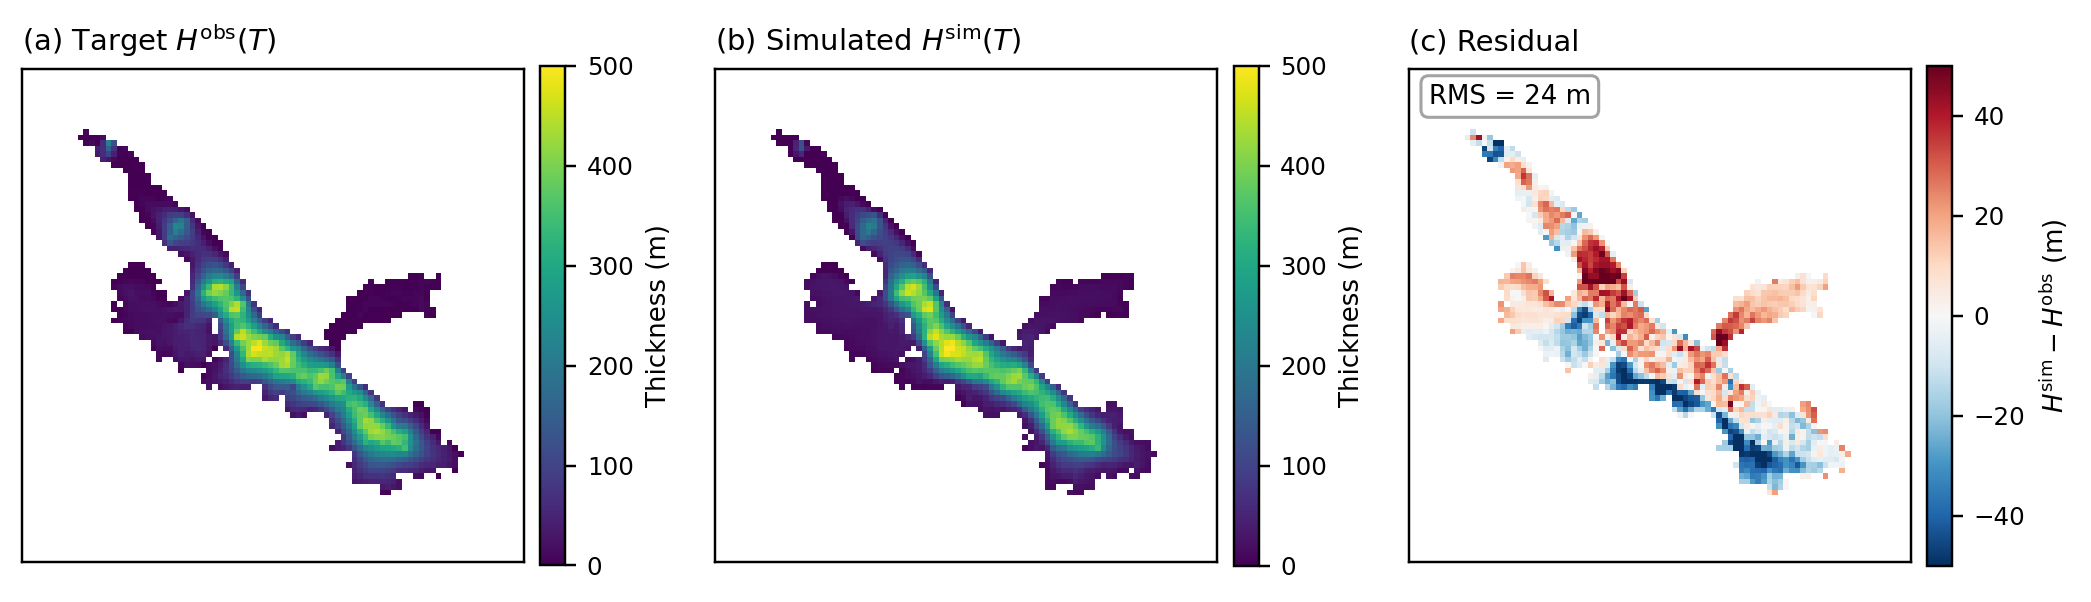
\includegraphics[width=\linewidth]{figs/argentiere_thk_comparison.png}
    \caption{End-of-window ice-thickness fit on Argentière Glacier ($T=2021$),
    all fields masked to the glacier footprint. (a)~Target thickness
    $H^\mathrm{obs}(\cdot, T)$ from the observed surface DEM and the calibrated
    bedrock; (b)~simulated thickness $H^\mathrm{sim}(\cdot, T)$ from the forward run
    under the inferred SMB profile; (c)~their residual
    $H^\mathrm{sim}-H^\mathrm{obs}$ (RMS $24\,\mathrm{m}$ over the glacier). The
    residual is small and largely unbiased; its spatially structured component
    reflects horizontal variability within elevation bands that the
    one-dimensional profile does not represent.}
    \label{fig:thk-comp}
\end{figure}

% --- TABLE PLACEHOLDER --------------------------------------------------
\begin{table}
    \centering
    \caption{Validation of inferred SMB against the GLACIOCLIM stake
    network on Argentière Glacier (main trunk + Améthystes tributary)
    over 2012--2021. The three baselines are the modelling approaches
    of \citet{kneib2024}, evaluated against the same set of stakes.}
    \label{tab:rmse}
    \begin{tabular}{lc}
        \hline
        Method & RMSE [m\,w.e.\,yr$^{-1}$] \\
        \hline
        F2019 \citep{kneib2024}            & 0.50 \\
        SIA \citep{kneib2024}              & 0.67 \\
        IGM-distributed \citep{kneib2024}  & 0.85 \\
        \textbf{Ours (1D AD inversion)}    & \textbf{0.454} \\
        \hline
    \end{tabular}
\end{table}
% ------------------------------------------------------------------------
% ------------------------------------------------------------
\subsection{Transfer to glaciers without thickness data: Great Aletsch and Rhône}
\label{sec:transfer}

To test whether the method transfers to glaciers lacking thickness observations,
we applied the identical two-step pipeline to Great Aletsch (2009--2017) and
Rhône (2007--2016), changing only the input data: no re-tuning of the
regularisation, optimiser or parameterisation was performed. Because neither
glacier has GPR coverage, the data assimilation is governed by the
surface-velocity misfit alone (Eq.~\ref{eq:da} with the thickness term omitted).
The calibrated states reproduce the observed surface velocities to
root-mean-square residuals of $9.9$ and $6.3$\,m\,yr$^{-1}$ on Aletsch and Rhône,
respectively (Table~\ref{tab:sens}), and the inversion converges to a comparable
geometry misfit as on Argentière (Fig.~\ref{fig:thk-transfer}).

\begin{figure}
  \centering
  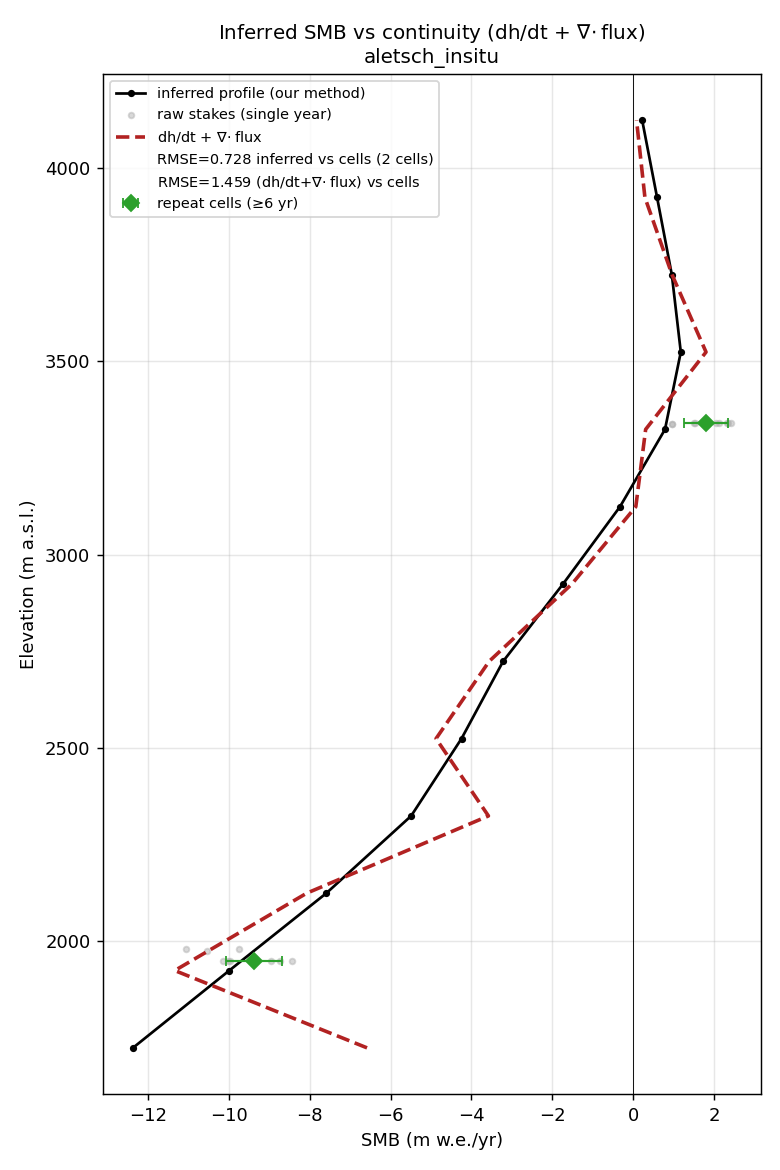
\includegraphics[width=0.45\linewidth]{figs/smb_vs_continuity_aletsch.png}
  \hfill
  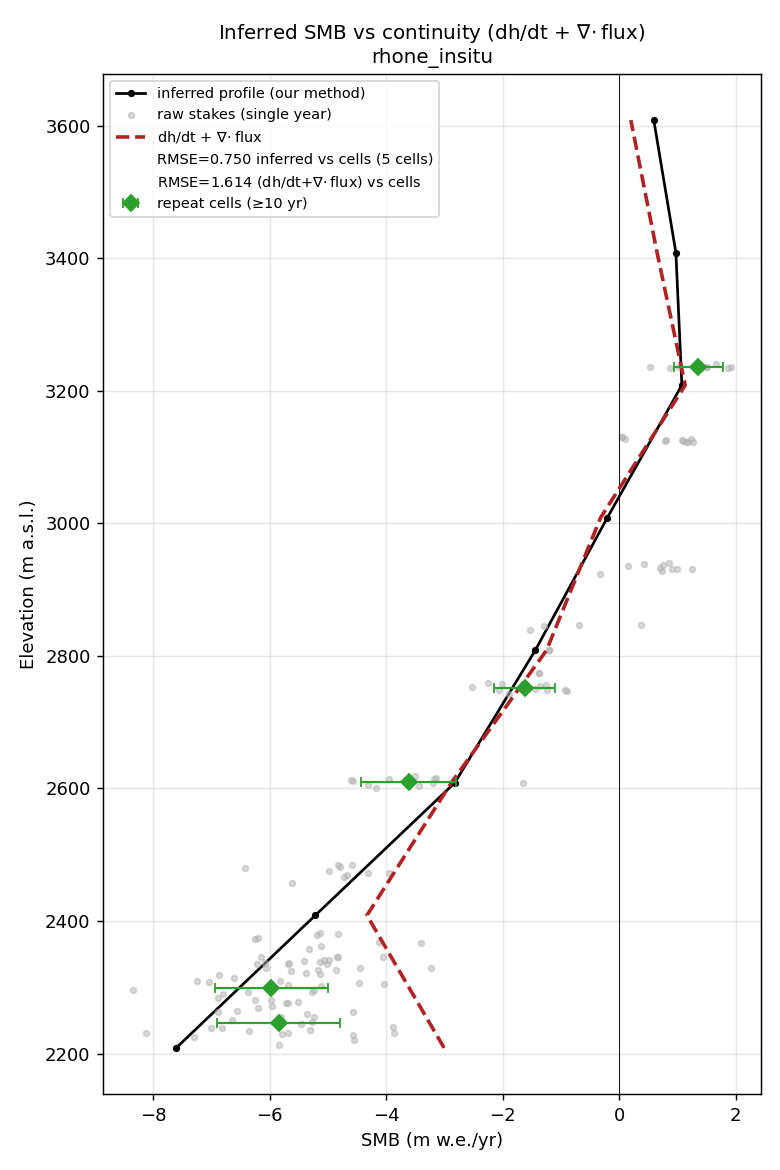
\includegraphics[width=0.45\linewidth]{figs/smb_vs_continuity_rhone.png}
  \caption{Inferred SMB profile (black) for (a)~Great Aletsch and (b)~Rhône,
    compared against in situ stake measurements and against the continuity
    estimate $\mathrm{d}h/\mathrm{d}t + \nabla\!\cdot\mathbf{q}$ (dashed),
    obtained with the stationary data-assimilation flux divergence. Faint grey
    dots are raw single-year stake readings; green diamonds are multi-year
    repeat-cell means ($\pm$ interannual standard deviation), the validation
    targets. The inferred profile tracks the repeat-cell means across the whole
    elevation range, whereas the continuity estimate departs strongly in the
    ablation zone, where the stationary flux divergence is least representative.}
  \label{fig:smb-continuity}
\end{figure}

The inferred profiles (Fig.~\ref{fig:smb-continuity}) are smooth and
monotonically increasing with elevation on both glaciers, from strongly negative
balances at the tongue to positive values in the accumulation area, and reproduce
the multi-year repeat-cell stake means---two cells on Aletsch and
five on Rhône---with root-mean-square errors of
$0.73$ and $0.75$\,m\,w.e.\,yr$^{-1}$
(Table~\ref{tab:transfer}). These values are consistent with the Argentière
benchmark despite the absence of any thickness constraint, confirming that the
velocity-calibrated dynamical state is sufficient to recover the elevation
structure of the SMB.

Figure~\ref{fig:smb-continuity} also makes concrete the mass-conservation
argument of Sect.~\ref{sec:sota}. The dashed curve is the SMB that the continuity
equation yields when the flux divergence is taken as stationary, exactly as in
flux-divergence inversions. On both glaciers this estimate is markedly noisier
than the inferred profile and diverges in the ablation zone---most severely on
Rhône, where the dense, fast-thinning tongue drives the stationary divergence far
from the stake means---raising the repeat-cell RMSE to $1.46$ and $1.61$\,m\,w.e.\,yr$^{-1}$
(Table~\ref{tab:transfer}). Because our forward model integrates the
mass-conservation law directly and recomputes the flux divergence from the
evolving geometry at every step, the inferred profile requires no spatial
smoothing and remains mass-consistent throughout, roughly halving the
ablation-zone error relative to the stationary-flux estimate.

\begin{table}
  \caption{Sensitivity of the inferred SMB to the basal sliding coefficient $c$
    on the two velocity-only Swiss glaciers, with the rate factor $A$ held fixed.
    \emph{velsurf} is the data-assimilation surface-velocity misfit---the only
    selector available without stakes---while RMSE is the independent validation
    against multi-year repeat-cell stake means ($n$ cells per glacier). Column
    minima per glacier in bold.}
  \label{tab:sens}
  \centering
  \begin{tabular}{lcccc}
    \toprule
    $c$ & velsurf & $\bar{b}$ & ELA & RMSE \\
    (MPa) & (m\,yr$^{-1}$) & (m\,w.e.\,yr$^{-1}$) & (m\,a.s.l.) & (m\,w.e.\,yr$^{-1}$) \\
    \midrule
    \multicolumn{5}{l}{\textit{Great Aletsch}\quad($A=182.1$\,MPa$^{-3}$\,yr$^{-1}$;\ $n=2$)} \\
    0.098 & 15.59          & $-4.00$ & 3009 & 2.83 \\
    0.154 & \textbf{9.94}  & $-3.34$ & 3127 & 0.90 \\
    0.199 & 10.14          & $-3.17$ & 3183 & \textbf{0.73} \\
    0.269 & 11.36          & $-2.89$ & 3198 & 0.86 \\
    \midrule
    \multicolumn{5}{l}{\textit{Rhône}\quad($A=78.0$\,MPa$^{-3}$\,yr$^{-1}$;\ $n=5$)} \\
    0.090 & 7.66          & $-1.62$ & 2940 & 0.95 \\
    0.120 & \textbf{6.34} & $-1.88$ & 2957 & 0.81 \\
    0.154 & 6.40          & $-2.05$ & 2994 & 1.25 \\
    0.199 & 6.84          & $-1.72$ & 2997 & \textbf{0.32} \\
    0.269 & 7.35          & $-1.72$ & 2995 & \textbf{0.32}? \\ % 0.39
    \bottomrule
  \end{tabular}
\end{table}


% ------------------------------------------------------------
\subsection{Sensitivity to the basal sliding coefficient}\label{sec:sensitivity}

The basal sliding coefficient $c$ is calibrated by data assimilation, but on a
glacier without thickness or stake data its value rests on the surface-velocity
misfit alone. To quantify how this choice propagates into the inferred SMB---and
whether velocity data are sufficient to make it---we repeated the inversion on
Aletsch and Rhône over a range of $c$, holding the rate factor fixed at each
glacier's adopted value (Table~\ref{tab:sens}). Both glaciers carry stake
networks, so the stake RMSE provides an independent ground truth against the only
selector available operationally, the data-assimilation velocity misfit
(\emph{velsurf}).

Three results emerge. First, \emph{velsurf} is U-shaped in $c$ and reliably
rejects the corrupting regime: its worst value lies at the high-sliding extreme
(lowest $c$), which on Aletsch is also where the SMB is most strongly biased---an
over-deep ablation tongue with mean SMB $-4.00$\,m\,w.e.\,yr$^{-1}$ and stake
RMSE $2.83$. Minimising the velocity misfit therefore keeps the inversion out of
the regime that most corrupts the profile. Second, \emph{velsurf} has a flat
minimum and cannot pin a single optimum: the velocity-selected coefficient and
the stake-optimal one are adjacent but not identical ($c=0.154$ vs $0.199$ on
Aletsch, $0.120$ vs $0.199$ on Rhône), with the stake optimum lying within
$2\,\%$ (Aletsch) and $8\,\%$ (Rhône) of the velocity minimum---inside the misfit
noise. On Rhône the stake RMSE even varies non-monotonically across the basin
($0.32$--$1.25$\,m\,w.e.\,yr$^{-1}$), confirming that velocity cannot resolve
within-band differences. The data thus constrain $c$ to a band, not a point.
Third, this residual uncertainty maps almost entirely onto the ablation zone:
across the flat velocity basin the accumulation-area profile is essentially
unchanged, while the tongue SMB and hence the equilibrium-line altitude shift
(3127--3198\,m on Aletsch; $\sim$40\,m on Rhône), and the glacier-wide mean SMB
ranges over $-3.34$ to $-2.89$ (Aletsch) and $-2.05$ to $-1.72$\,m\,w.e.\,yr$^{-1}$
(Rhône) (Fig.~\ref{fig:sens}).

\begin{figure}
  \centering
  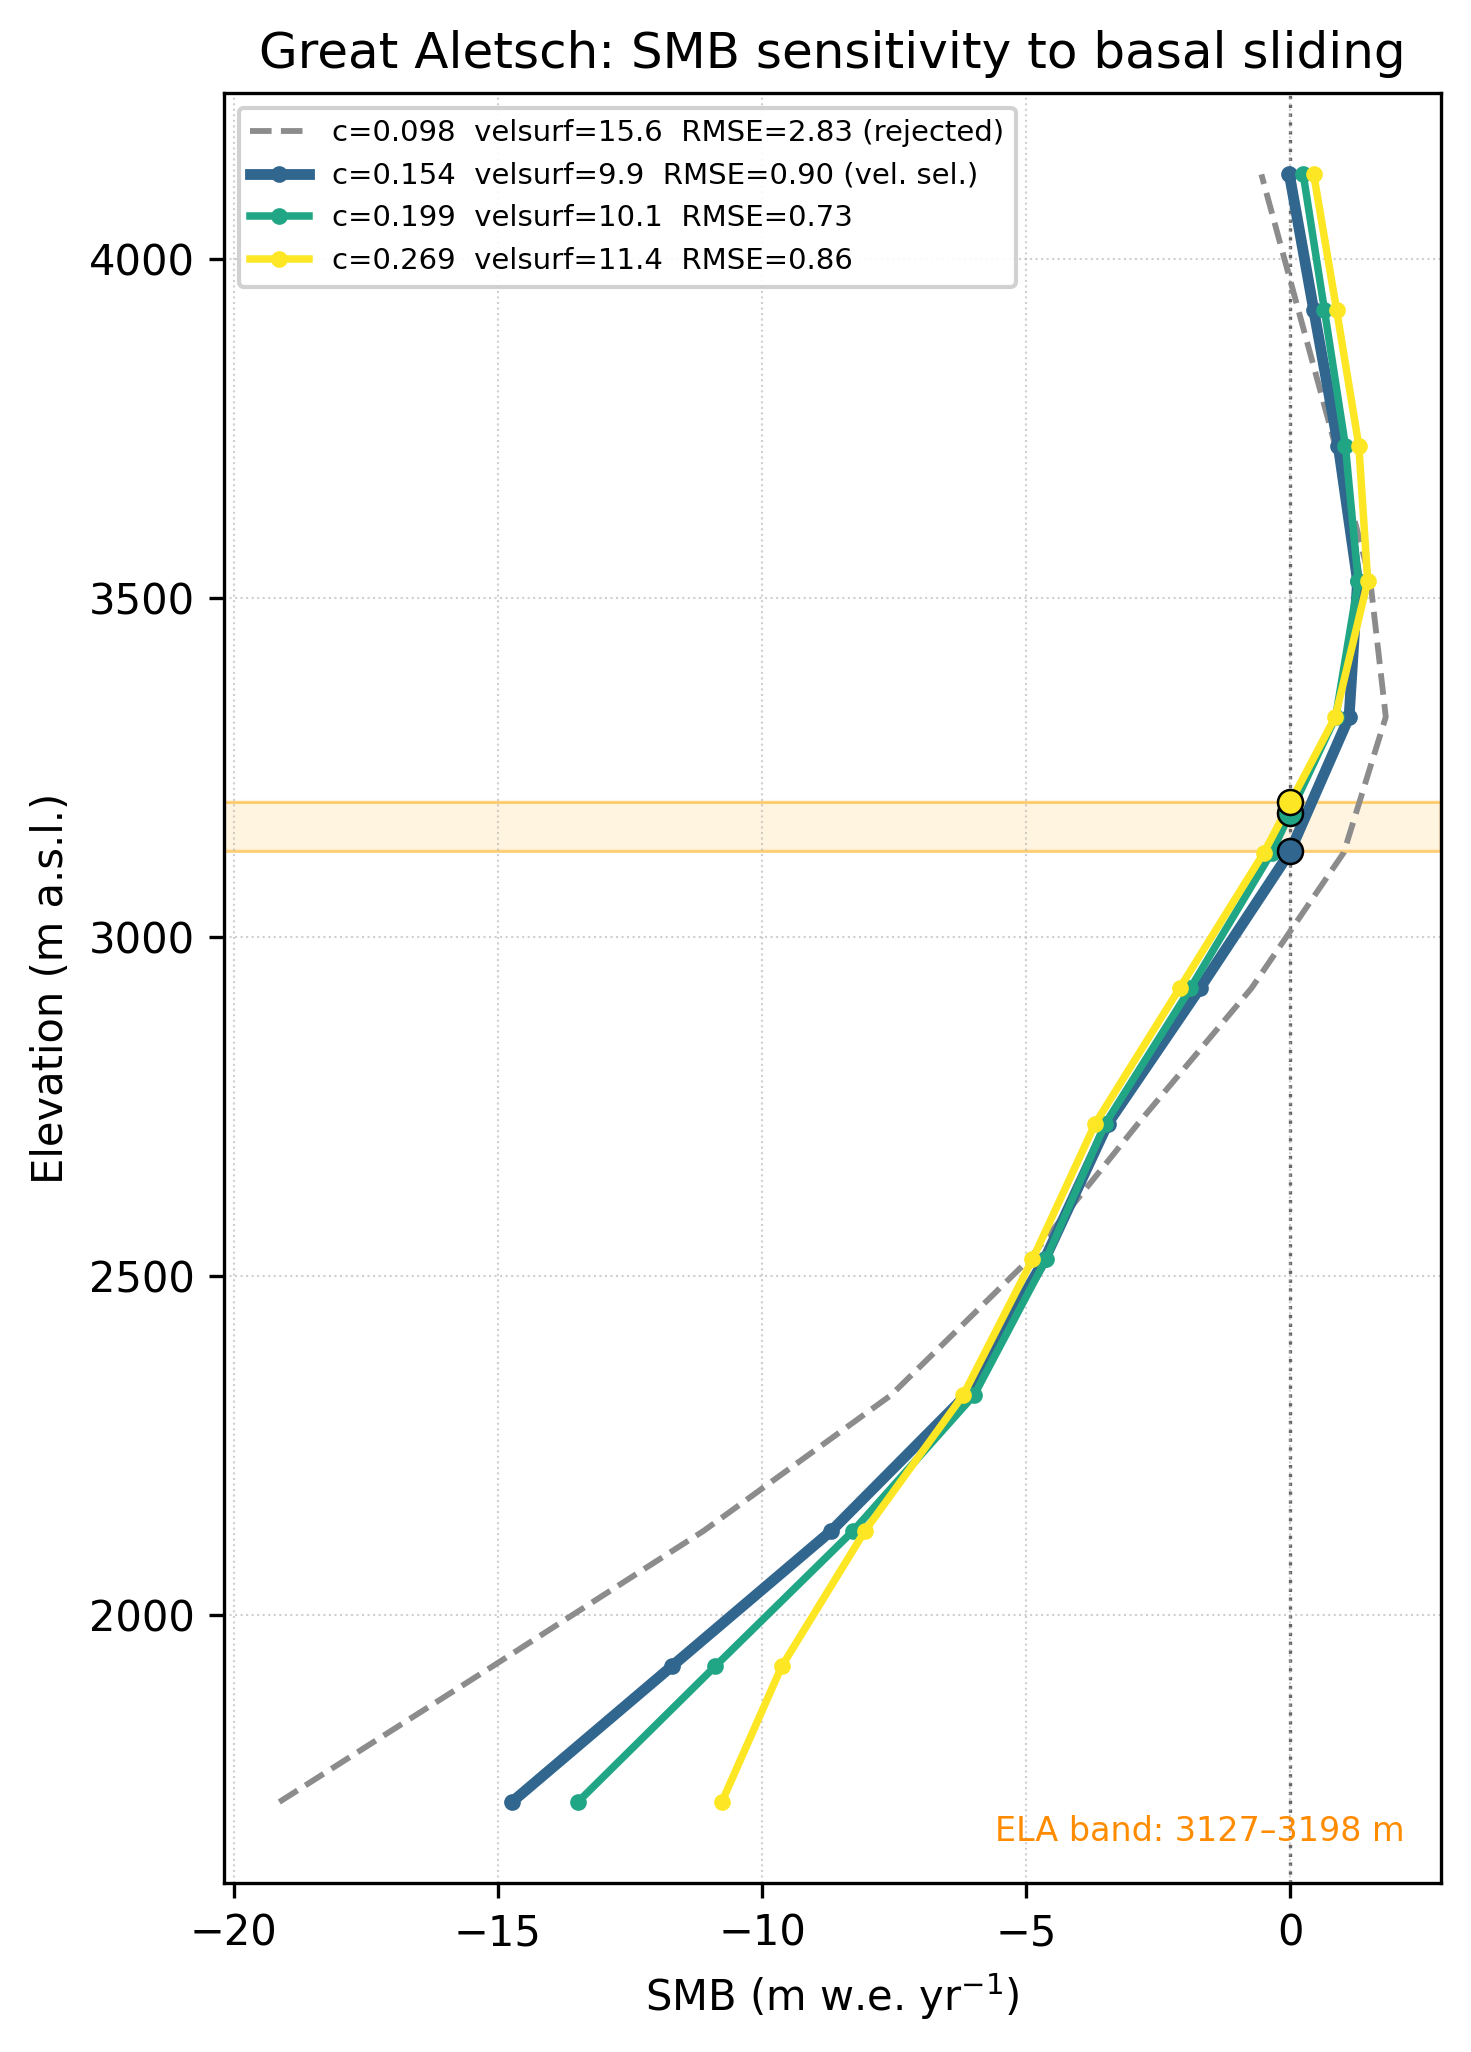
\includegraphics[width=0.45\linewidth]{figs/sens_slidingco_aletsch.png}
  \hfill
  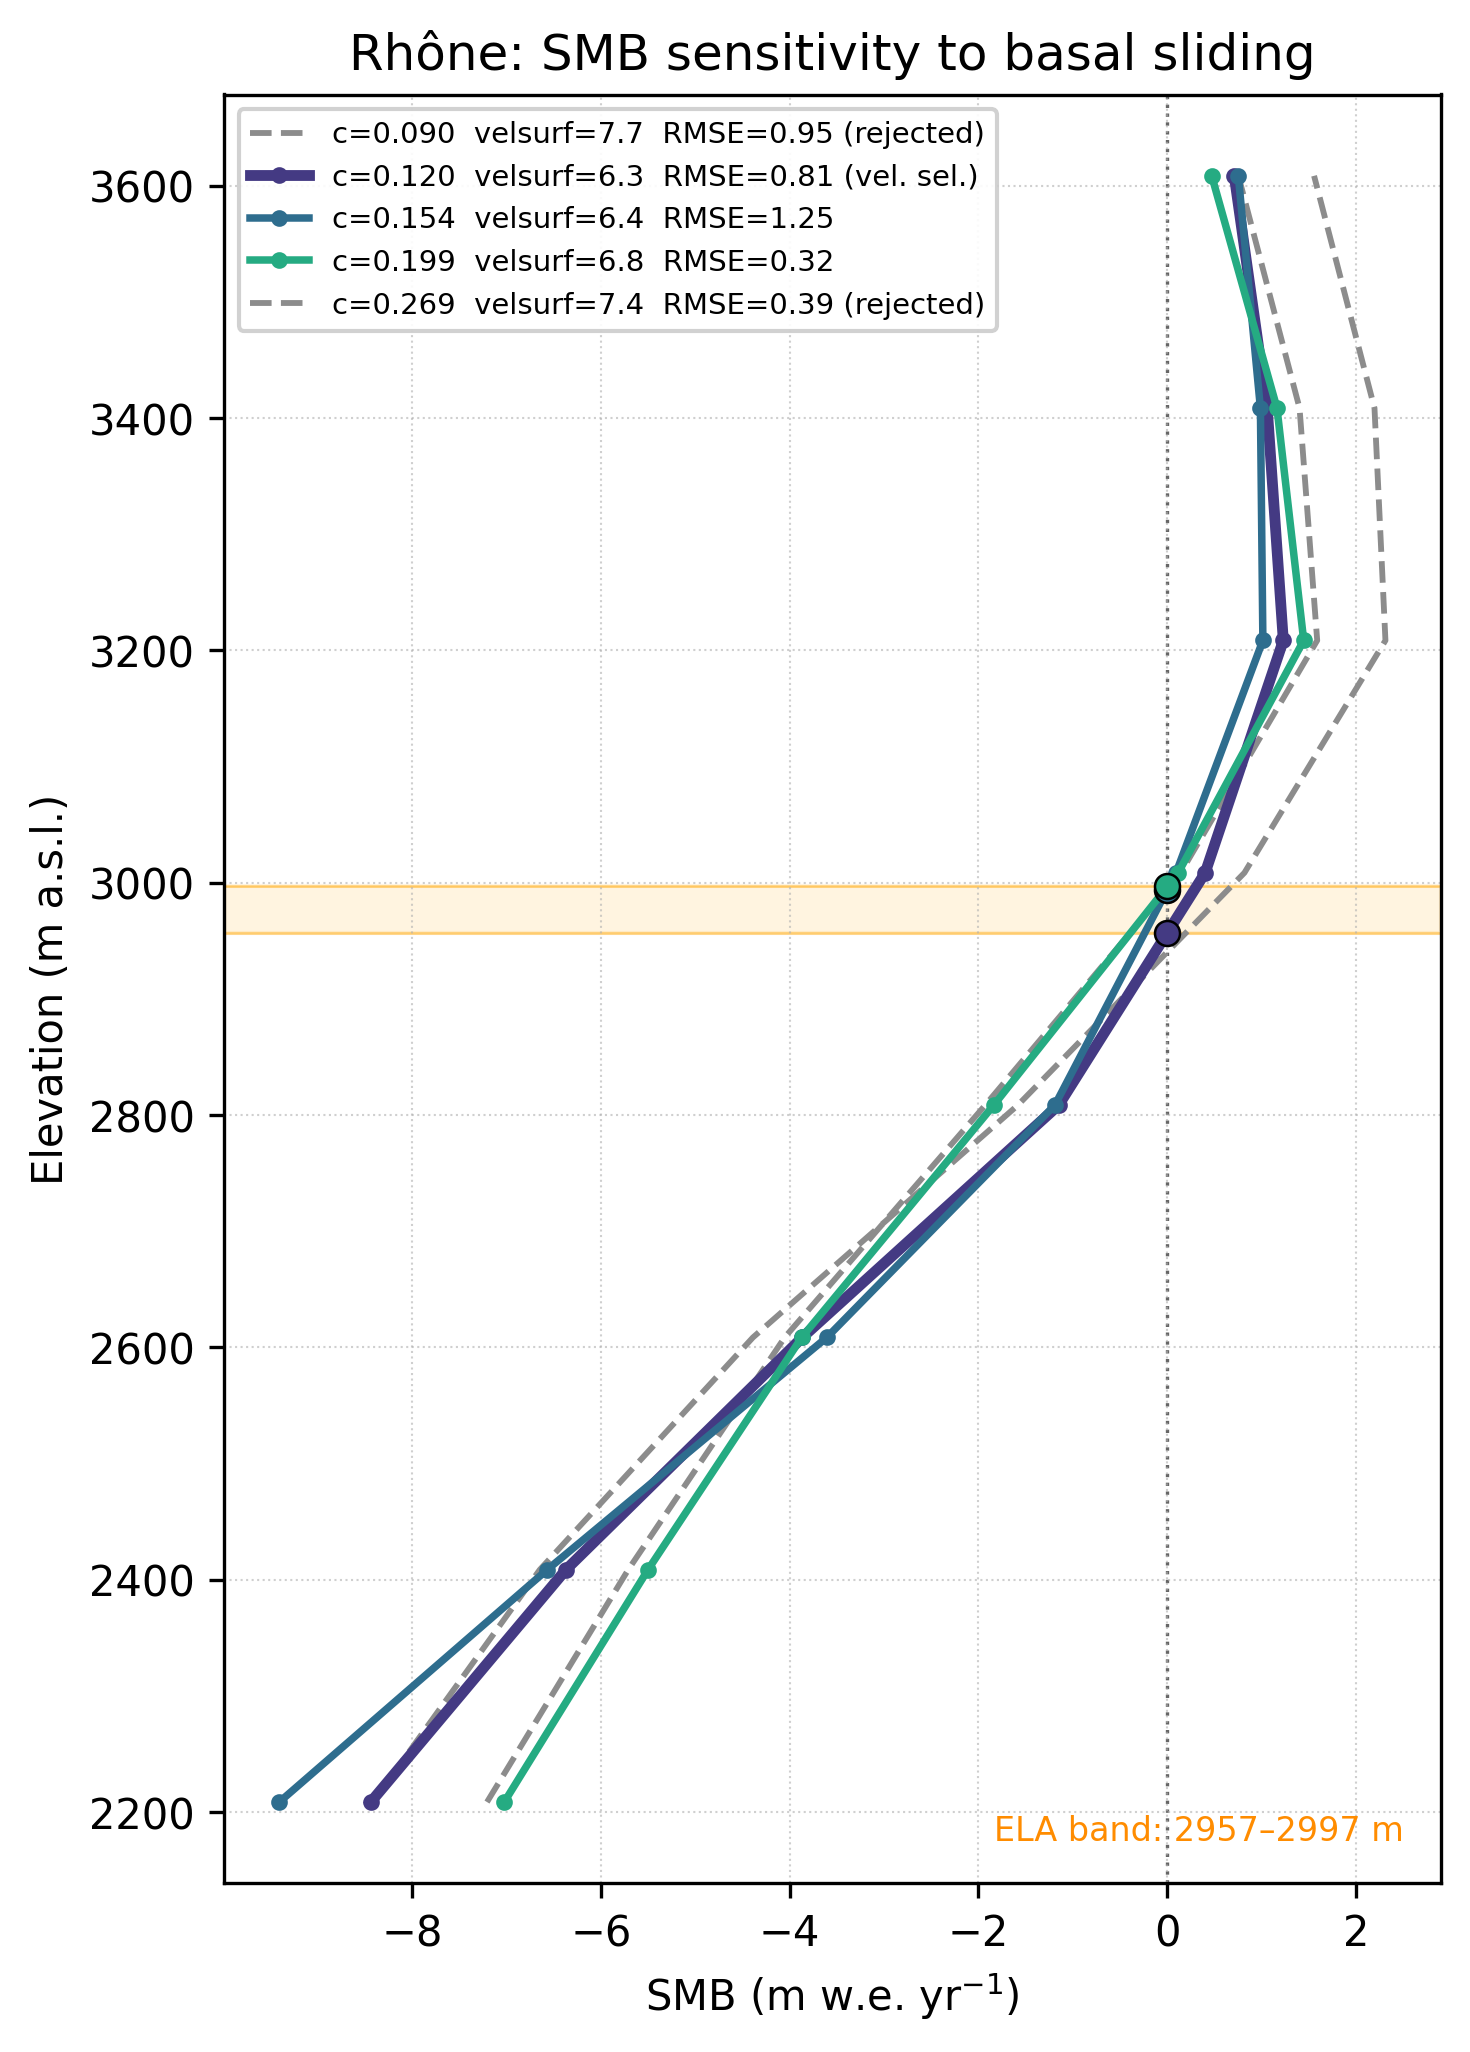
\includegraphics[width=0.45\linewidth]{figs/sens_slidingco_rhone.png}
  \caption{Inferred SMB profiles for (a)~Great Aletsch and (b)~Rhône over the
    range of basal sliding coefficients within the velocity-misfit basin
    (Table~\ref{tab:sens}). The profiles coincide in the accumulation area and
    diverge only at the ablation tongue, so the residual sliding uncertainty
    translates into an equilibrium-line altitude band (shaded) rather than a
    whole-profile bias.}
  \label{fig:sens}
\end{figure}

Taken together, these results define a velocity-only procedure for stake-free
glaciers: adopt the sliding coefficient at the velocity-misfit minimum, but
propagate the two to three coefficients within $\sim$10--15\,\% of that minimum
into an SMB and equilibrium-line uncertainty band, tight in the accumulation area
and widening at the tongue. The operational implications are taken up in
Sect.~\ref{sec:discussion}. The rate factor was held at a temperature prior
throughout; because it trades off with $c$ in the velocity field, the band is
conditional on that prior, which is the weaker of the two knobs.